\section{Google Games}
Google Play Games (GGames from now on) provides a way to easily manage every detail of a game. By using it, users may complete achievements and quests, see ranks and experience a consistent feeling thorough difference devices. At the administrator side, it allows us to configure everything by using the Google Play Console.

We use GGames for a number of purposes. First of all, since QuizFight is a game, we define different achievements with an increasing difficulty level. Examples are ''\textit{Win 100 duels}'', ''\textit{Answer correctly to 1000 questions}'' or ''\textit{Score 45 points in a duel}''. As usual, by unlocking achievements the users gain experience. We also collect information about different events, such as the number of correct answers, the number of duels, or rounds, played and so on. Using GGames for storing those statistics is useful because it provides a very easy interface and allows us not to reinvent the wheel by reimplementing everything from scratch. The most important service we used is \textbf{Saved Games}, as discussed below.

\subsection{Sign In}

\subsection{Saved Games}
The most important service used in QuizFight is named \textbf{Saved Games}. It gives us a convenient way to save our players' game progression to Google's servers. We can then retrieve the saved game data to allow returning players to continue a game at their last save point from any device. The Saved Games service makes it possible to synchronize a player's game data across multiple devices. For example, if you have a game that runs on Android, you can use the Saved Games service to allow a player to start a game on their Android phone, and then continue playing on a tablet without losing any of their progress. Even if we save anyway the data on our server's database, Saved Games allows us to limit the network traffic with the server and provides an easy way to store the information even if the device has no connectivity. In fact, if the device is disconnected, Saved Games stores locally the data to be saved and, at the very first reconnection, it sends that to Google's servers.

A saved game consists of two parts:
\begin{itemize}
	\item an unstructured binary blob: this data can represent whatever we choose, and our game is responsible for parsing and writing to it;
	\item structured metadata: additional properties associated with the binary data that allow GGames services to visually present Saved Games in the default Saved Games list user interface (UI), and to present useful information in the GGames app (for example, last updated timestamp).
\end{itemize}
A game can write an arbitrary number of Saved Games for a single player, subject to user quota, so there is no hard requirement to restrict players to a single save file. Every game may save up to 3MB blobs. They are stored in the player's Google Drive space. Google ensures read/write isolation: only QuizFight is able to read QuizFight's saved data.

Figure~\ref{fig:saved-games-hierarchy} shows how we interact with Saved Games.
\begin{figure}
	\centering
	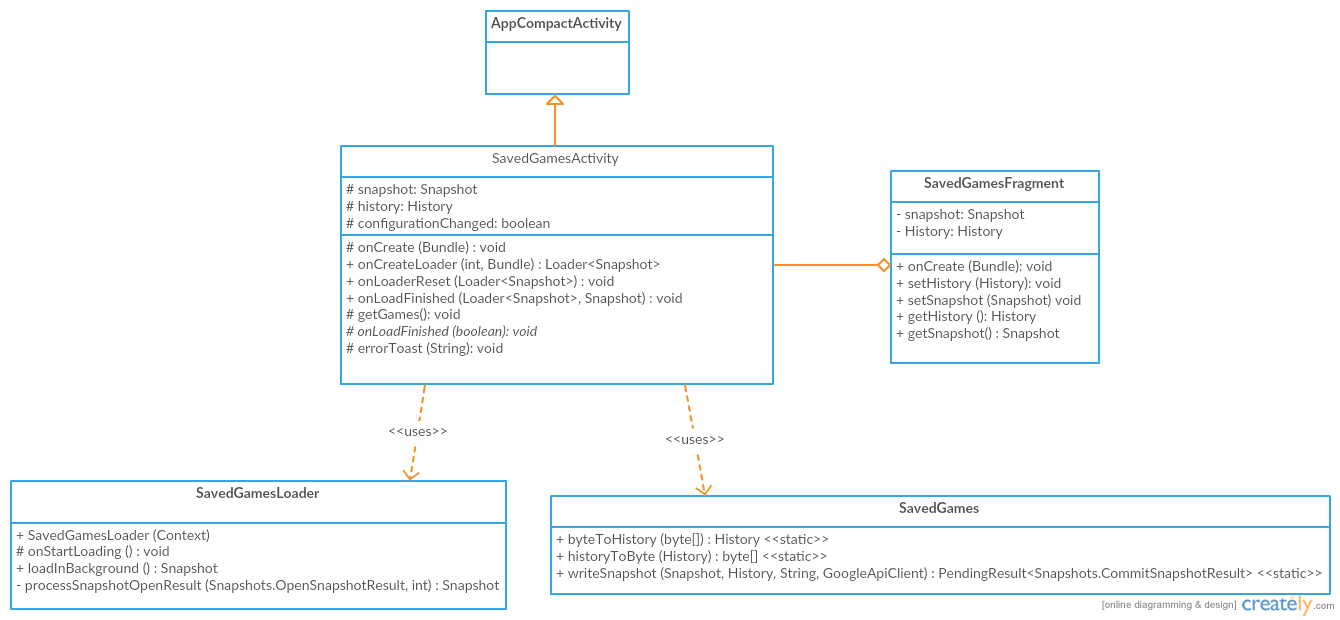
\includegraphics[width=1\linewidth]{SavedGamesHierarchy}
	\caption[Saved Games Hierarchy]
	\label{fig:saved-games-hierarchy}
\end{figure}
